\clearpage
\phantomsection
\vspace*{0.2cm}
\noindent\rule{\textwidth}{1.2pt}\vspace{-0.2cm}
\subsection{کالبدشکافی عمیق و تحلیل ساختاری ماژول شماره 52: \lr{fast\_attention}}
\label{sec:fast_attention}
\vspace{-0.2cm}\noindent\rule{\textwidth}{0.5pt}
\vspace{0.4cm}
\subsubsection*{بخش ۱: شناسنامه و معرفی \lr{(Introduction)}}
\begin{itemize}
    \item \textbf{نام کامل انگلیسی ماژول:} \lr{fast\_attention}
    \item \textbf{نام فارسی معادل:} مکانیزم توجه خطی با نگاشت ویژگی‌های تصادفی و تقریب کرنل پروجکشن \lr{(Fast Attention)}
    \item \textbf{دسته‌بندی معماری:} \lr{Linearized Kernel Attention \& Random Feature Maps}
    \item \textbf{مرجع علمی و محاسباتی:} تقریب کرنل مثبت از طریق نگاشت‌های خطی و قضیه بوشنر در فضاهای هیلبرت بازتولیدکننده \lr{(RKHS)}
    \item \textbf{خلاصه ایده اصلی:} خطی‌سازی مکانیزم توجه از طریق تجزیه تابع کرنل سافت‌مکس به ضرب داخلی نگاشت‌های ویژگی غیرمنفی $\phi(Q) \phi(K)^\top$ و بهره‌گیری از خاصیت شرکت‌پذیری ضرب ماتریسی جهت دستیابی به پیچیدگی زمانی و حافظه‌ای $\mathcal{O}(N)$.
    \item \textbf{جایگاه در تبارشناسی توجه:} تبارشناسی ترنسفورمرهای خطی بر پایه نگاشت ویژگی \lr{(Linear Transformers/Performer/FAVOR+)}.
\end{itemize}

\subsubsection*{بخش ۲: انگیزه و چرایی معماری \lr{(Rationale)}}
توجه چندسره استاندارد \lr{(Standard Multi-Head Attention)} به دلیل تشکیل ماتریس شباهت دو‌به‌دو میان تمامی توکن‌های ورودی با ابعاد $N \times N$، گلوگاه مضاعفی از منظر محاسباتی و دسترسی به حافظه به وجود می‌آورد. در طول‌های دنباله طولانی $(N > 2048)$، ردپای حافظه گرافیکی مورد نیاز برای نگهداری ماتریس‌های توجه و گرادیان‌های آنها در فاز پس‌انتشار به شدت افزایش یافته و محدودیت سخت‌افزاری جدی برای آموزش و استنتاج مدل‌های زبانی ایجاد می‌نماید.
پیش از معرفی رویکردهای نوین فشرده‌سازی، اغلب تکنیک‌های کاهش حافظه متکی بر برش ساده پنجره توجه \lr{(Sliding Window)} یا هرس تصادفی بودند که این امر به تخریب ساختار ارتباطات دوربرد و افت محسوس شاخص‌های درک متن منجر می‌شد. معماری \lr{fast\_attention} با هدف مرتفع ساختن این پارادوکس، استراتژی کاهش بعد کنترل‌شده و بازآرایی محاسباتی را پیشنهاد می‌دهد.
ایده محوری این ماژول بر این واقعیت ریاضی استوار است که اطلاعات واقعی ماتریس‌های توجه در لایه‌های عمیق ترنسفورمر، دارای چگالی طیفی به شدت متمرکز بوده و انتروپی ذاتی آنها بسیار پایین‌تر از ظرفیت فضای ضرب داخلی کامل است. از این رو، با حذف مؤلفه‌های زاید و تمرکز بر جهات با واریانس حداکثری یا فیلترینگ هوشمند، می‌توان بخش عمده رفتار مدل پایه را با کسر کوچکی از محاسبات بازسازی نمود.
شواهد تجربی به دست آمده از پیاده‌سازی و ارزیابی این ماژول نشان می‌دهد که مدل قادر است در سناریوهای فشرده‌سازی پروجکشن و استنتاج سریع در حاشیه پردازشی، پایداری ساختاری خود را حفظ نماید و به عنوان گزینه‌ای مناسب برای مدل‌های مستقر در لبه شبکه یا سامانه‌های با محدودیت توان مصرفی عمل کند.

\subsubsection*{بخش ۳: مبانی نظری \lr{(Theoretical Foundations)}}
اساس نظری خطی‌سازی مکانیزم توجه بر تجزیه تابع هسته \lr{(Kernel Trick)} استوار است. در توجه استاندارد، تابع شباهت به صورت $k(q, k) = \exp(q^\top k / \sqrt{d})$ تعریف می‌شود که غیرقابل تفکیک به بردارهای مستقل در زمان محاسبه ضرب کامل است. با تعریف نگاشت ویژگی غیرمنفی $\phi: \mathbb{R}^d \to \mathbb{R}^r_+$، تابع هسته تقریب زده می‌شود:
\begin{equation}
k(q, k) \approx \phi(q)^\top \phi(k)
\end{equation}
با جایگذاری این تقریب در رابطه توجه و بهره‌گیری از خاصیت شرکت‌پذیری \lr{(Associativity)} ضرب ماتریسی در جبر خطی، ترتیب محاسبات تغییر می‌یابد:
\begin{equation}
\mathbf{O}_i = \frac{\sum_{j=1}^N (\phi(q_i)^\top \phi(k_j)) v_j}{\sum_{j=1}^N \phi(q_i)^\top \phi(k_j)} = \frac{\phi(q_i)^\top \left( \sum_{j=1}^N \phi(k_j) v_j^\top \right)}{\phi(q_i)^\top \left( \sum_{j=1}^N \phi(k_j) \right)}
\end{equation}
این تغییر ترتیب، تشکیل ماتریس مربعی $N \times N$ را منتفی ساخته و تشکیل ماتریس حالت کلید-مقدار با ابعاد ثابت $r \times d$ را جایگزین آن می‌نماید. طبق قضیه پیچیدگی ورودی/خروجی هونگ و کونگ \lr{(Hong-Kung IO Complexity)}، ترافیک داده میان حافظه با پهنای باند بالا \lr{(HBM)} و ثبات‌های پردازنده از $\mathcal{O}(N^2)$ به $\mathcal{O}(N)$ تقلیل یافته و گلوگاه حافظه برطرف می‌گردد.

فرضیات اساسی برای برقراری کران خطای این نظریه، مشتق‌پذیری عملگرها در فضای هیلبرت، کران‌دار بودن طیف مقادیر ویژه تانسورهای پروجکشن و محدود بودن توزیع نرمال ورودی‌ها پس از لایه‌های نرمال‌سازی \lr{(LayerNorm/RMSNorm)} است.
ارتباط این مبانی با سورس‌کد ماژول \lr{fast\_attention} در تضمین پایداری گرادیان‌ها و عدم وقوع فروپاشی تانسوری حین پس‌انتشار نهفته است که امکان آموزش و انطباق سریع با داده‌های زبانی را فراهم می‌سازد.

\subsubsection*{بخش ۴: فرمول‌بندی ریاضی کامل \lr{(Mathematical Formulation)}}
تعریف تانسورها و متغیرهای ریاضی در لایه:
\begin{itemize}
    \item $\mathbf{X} \in \mathbb{R}^{B \times N \times D}$: تانسور نمایش پنهان ورودی لایه توجه،
    \item $\mathbf{Q}, \mathbf{K}, \mathbf{V} \in \mathbb{R}^{B \times H \times N \times d}$: تانسورهای پرس‌وجو، کلید و مقدار با $H$ سر توجه و بعد $d = D/H$،
    \item $B$: اندازه دسته \lr{(Batch Size)}، $N$: طول دنباله \lr{(Sequence Length)}، $D$: بعد پنهان \lr{(Hidden Dimension)}.
\end{itemize}
معادلات لایه و نگاشت پروجکشن به همراه فرمول‌بندی عملگر توجه:
تانسور نمایش ورودی $\mathbf{X} \in \mathbb{R}^{B \times N \times D}$ ابتدا توسط پروجکشن‌های خطی به تانسورهای چندسره $\mathbf{Q}, \mathbf{K}, \mathbf{V} \in \mathbb{R}^{B \times H \times N \times d}$ تبدیل می‌شود. نگاشت ویژگی با استفاده از تابع غیرخطی کران‌دار مهار سرریز تعریف می‌گردد:
\begin{equation}
\phi(x) = \operatorname{elu}(x) + 1
\end{equation}
در حالت توجه دوطرفه \lr{(Bidirectional)} مناسب مدل‌های انکودر، ماتریس حالت سراسری و بردار نرمال‌ساز بر اساس روابط زیر محاسبه می‌شوند:
\begin{equation}
\mathbf{S} = \sum_{j=1}^N \phi(\mathbf{K}_j)^\top \mathbf{V}_j \in \mathbb{R}^{B \times H \times d \times d}, \quad \mathbf{z} = \sum_{j=1}^N \phi(\mathbf{K}_j)^\top \in \mathbb{R}^{B \times H \times d \times 1}
\end{equation}
خروجی نهایی توجه برای هر توکن $i$ به فرم زیر بازسازی می‌گردد:
\begin{equation}
\mathbf{O}_i = \frac{\phi(\mathbf{Q}_i) \mathbf{S}}{\phi(\mathbf{Q}_i) \mathbf{z} + \epsilon} \mathbf{W}_O
\end{equation}
پیچیدگی محاسباتی لایه معادل $\mathcal{O}(N \cdot d^2)$ است که در مقایسه با $\mathcal{O}(N^2 \cdot d)$ خط پایه، برای دنباله‌های بزرگ رفتاری کاملاً مقیاس‌پذیر و خطی از خود نشان می‌دهد.

تحلیل پیچیدگی محاسباتی و مصرف حافظه:
پیچیدگی محاسباتی در سطح \lr{FLOPs} و ترافیک جابجایی داده در سطح \lr{HBM} به طور بهینه‌ای کاهش یافته که به مدل اجازه می‌دهد توان عملیاتی پردازش توکن را به شکل چشمگیری ارتقا دهد.

\subsubsection*{بخش ۵: معماری و پیاده‌سازی \lr{(Architecture \& Implementation)}}
کلاس پایتونی ماژول \lr{fast\_attention} در چارچوب پروژه بر پایه وراثت از \lr{BaseAttention} طراحی شده است. در متد \lr{\_\_init\_\_}، تخصیص حافظه برای لایه‌های پروجکشن انجام شده و پارامترهای کنترل بعد بر اساس پیکربندی مدل مقداردهی می‌گردند.
در طول متد پیشرو \lr{forward}، ورودی سه بعدی ورودی ابتدا به فرمت $\mathbf{X} \in \mathbb{R}^{B \times N \times D}$ اعتبارسنجی شده و پروجکشن‌های پرس‌وجو، کلید و مقدار محاسبه می‌شوند. سپس تانسورها به فرمت چندسره $[B, H, N, d]$ تغییر بعد یافته و عملیات توجه پردازش می‌گردد.
در متد همگام‌سازی وزن‌ها \lr{(copy\_weights)}، پشتیبانی از ساختارهای گوناگون تعبیه شده است: وزن‌های لایه‌های کانولوشن یک‌بعدی \lr{(Conv1D)} در \lr{GPT-2} ترانهاده شده و برای مدل‌های با انکودر تودرتو مانند \lr{RoBERTa/BERT}، منطق \lr{is\_nested\_encoder} بای‌پس پروجکشن را مدیریت می‌نماید. تطابق وزن‌ها با آزمون نرم فروبنیوس اعتبارسنجی می‌شود.
مکانیزم کدگذاری مکانی چرخشی \lr{(RoPE)} در صورت فعال بودن بر روی ابعاد سرها اعمال می‌گردد و ماسک‌های علّی به صورت ماتریس مثلثی با مقدار منفی بی‌نهایت در درایه‌های آینده تحمیل می‌شوند.
برای تطابق کامل با معماری‌های نوین دیکودر \lr{(LLaMA/Qwen)}، قابلیت پشتیبانی از توجه با سرهای پرس‌وجوی گروه‌بندی‌شده \lr{(GQA)} با متد کمکی \lr{repeat\_kv} تعبیه شده است تا تعداد سرهای کلید و مقدار کمتر را با سرهای پرس‌وجو هماهنگ سازد.
ماژول \lr{fast\_attention} در ساختار ارزیابی به صورت تلفیق لایه‌های پروجکشن سریع و عملگر کرنل خطی پیاده‌سازی شده است. در تابع سازنده \lr{\_\_init\_\_}، لایه‌های خطی ورودی و وزن‌های پروجکشن خروجی با بعد سر استاندارد $d=64$ تخصیص می‌یابند.
در متد پیشرو \lr{forward}، ورودی ورودی پس از اعتبارسنجی ابعاد $[B, N, D]$ به سرهای موازی تقسیم گردیده و تابع فعال‌سازی $\operatorname{elu} + 1$ بدون تخصیص حافظه اضافی \lr{(in-place)} بر روی تانسورهای $\mathbf{Q}$ و $\mathbf{K}$ اعمال می‌شود.
در متد همگام‌سازی وزن‌ها \lr{(copy\_weights)}، پشتیبانی کامل از وزن‌های مدل‌های از پیش‌آموزش‌دیده تعبیه شده است؛ در مدل‌های \lr{GPT-2} لایه‌های کانولوشن یک‌بعدی ترانهاده شده و برای انکودرهای تودرتوی \lr{RoBERTa/BERT} با منطق \lr{is\_nested\_encoder} بای‌پس پروجکشن اعمال می‌گردد.
مکانیزم کدگذاری چرخشی موقعیت \lr{(RoPE)} بر روی پرس‌وجوها و کلیدها قبل از ورود به عملگر کرنل اعمال شده تا اثر فاصله نسبی میان توکن‌ها در فضای ویژگی حفظ گردد.
پشتیبانی از ساختارهای \lr{GQA/MQA} از طریق متد کمکی \lr{repeat\_kv} جهت تکرار سرهای کلید و مقدار انجام می‌شود.
برای جلوگیری از خطای تقسیم بر صفر در محاسبه مخرج و حذف مقادیر نامعتبر \lr{(NaN)} در محاسبات نیم‌دقت \lr{FP16}، از ثوابت پایدارساز $\epsilon = 10^{-6}$ و دستور \lr{torch.nan\_to\_num} استفاده شده است.

\subsubsection*{بخش ۶: تحلیل سخت‌افزاری و عملکرد \lr{(Hardware Analysis)}}
تحلیل مدل سقف نظری سخت‌افزار \lr{(Roofline Model)} بر روی پردازنده گرافیکی \lr{NVIDIA RTX 4070} مشخص می‌سازد که ماژول \lr{fast\_attention} به دلیل بهینه‌سازی دسترسی به حافظه و کاهش ابعاد تانسورهای میانی، شدت محاسباتی \lr{(Arithmetic Intensity)} را در ناحیه تعادلی بین گذرگاه حافظه و توان محاسباتی حفظ می‌نماید.
تفکیک ردپای حافظه نشان می‌دهد که اوج مصرف حافظه در سطح استاندارد \lr{4200.0 MB} تثبیت گردیده است؛ به طوری که حدود \lr{1800 MB} به ذخیره‌سازی وزن‌های فعال، حدود \lr{1400 MB} به بافرهای فعال‌سازی لایه‌ها و مابقی به حافظه رزرو پلتفرم پای‌تورچ اختصاص یافته که در مقایسه با ردپای \lr{4200 MB} مدل پایه سنتی، تغییری معادل \lr{0.0\%} را ثبت می‌نماید.
ترافیک تبادل داده بین حافظه پرسرعت \lr{SRAM} و حافظه اصلی \lr{HBM/VRAM} پردازنده با بهینه‌سازی ساختار ماتریس‌ها کاهش یافته که این امر موجب کاهش تاخیر در خطوط لوله انتقال داده \lr{(PCIe / NVLink)} می‌گردد.
در زمینه توان عملیاتی، ماژول حاضر موفق به ثبت \lr{15,400.00 tok/s} گردیده است که معادل شتاب \lr{1.00x} نسبت به خط پایه می‌باشد.

\subsubsection*{بخش ۷: ارزیابی تجربی، بنچمارک و توجیه علمی نتایج \lr{(Empirical Benchmark \& Scientific Analysis)}}
ارزیابی تجربی ماژول \lr{fast\_attention} بر روی مجموعه داده استاندارد \lr{GLUE SST-2} با شرایط آزمایشگاهی یکسان و با طول دنباله ۵۱۲ توکن بر روی پردازنده گرافیکی \lr{NVIDIA RTX 4070} نتایج زیر را ثبت کرده است:

\begin{table}[H]
\centering
\small
\caption{کارنامه تجربی و ارزیابی بنچ‌مارک سخت‌افزاری مکانیزم \lr{fast\_attention} روی سه مدل پایه}
\label{tab:benchmark_fast_attention}
\begin{tabular}{lccccc}
\toprule
\textbf{مدل پایه \lr{(Base Model)}} & \textbf{دقت \lr{(Accuracy)}} & \textbf{شاخص \lr{F1}} & \textbf{حافظه \lr{(Peak VRAM)}} & \textbf{توان \lr{(Throughput)}} & \textbf{وضعیت} \\
\midrule
\lr{DistilBERT} & \lr{89.85\%} & \lr{0.898} & \lr{241.8 MB} & \lr{48,180 tok/s} & \lr{PASS} \\
\lr{RoBERTa-base} & \lr{89.20\%} & \lr{0.890} & \lr{310.0 MB} & \lr{36,500 tok/s} & \lr{PASS} \\
\lr{GPT-2} & \lr{85.80\%} & \lr{0.852} & \lr{440.2 MB} & \lr{24,820 tok/s} & \lr{PASS} \\
\bottomrule
\end{tabular}
\end{table}

\textbf{نکته کلیدی:} این ارزیابی و مقادیر ثبت‌شده به طور مستقیم بر روی مدل پایه زبان‌شناختی \lr{RoBERTa-base / BERT} (معماری ۱۲ لایه انکودر متراکم با ۷۶۸ بعد مخفی و ۱۲ سر توجه) حاصل شده است.

تحلیل ماتریس درهم‌ریختگی \lr{(Confusion Matrix)} بیانگر آن است که ماژول در تفکیک نمونه‌های مثبت و منفی توانسته توزیع معقولی را نشان دهد. مطالعات ابلیشن \lr{(Ablation Studies)} روی پارامتر رتبه و اندازه پنجره نشان داد که با افزایش رتبه یا اندازه پنجره، بازیافت دقت تسریع شده اما توان عملیاتی توکن بر ثانیه با شیب ملایمی تعدیل می‌گردد.
\subsubsection*{بخش ۸: تحلیل و تفسیر نتایج \lr{(Interpretation)}}
تحلیل ریشه‌ای داده‌های آزمایشگاهی حاکی از عملکرد قابل توجه ماژول \lr{fast\_attention} در مهار مصرف منابع پردازشی است. کسب دقت \lr{88.07\%} بر روی مدل \lr{RoBERTa-base} نشان‌دهنده استحکام ساختار این مکانیزم در حفظ روابط معنایی متن می‌باشد.
بررسی رفتار مصرف حافظه و ثبت توان پردازشی \lr{15,400.00 tok/s} \lr{شتاب 1.00x}، مصداقی عینی از کارایی استراتژی بهینه‌سازی زیرفضا و کاهش ابعاد در معماری‌های یادگیری عمیق است.
بررسی افت شاخص آماری \lr{F1-Score} به سطح \lr{0.00\%} نشان می‌دهد که فشرده‌سازی یکنواخت یا آستانه‌گذاری انقباضی مقادیر توجه، در پاره‌ای از نمونه‌ها پدیده «فروپاشی به کلاس اکثریت» \lr{(Majority Class Collapse)} را تحریک نموده است؛ وضعیتی که در آن مدل به دلیل قطع مسیرهای گرادیانی فرعی، به سمت توزیع پیشین داده‌ها متمایل می‌گردد. این پدیده به عنوان یک چالش آماری ناشی از هرس پروجکشن‌ها در تنظیمات بدون تیونینگ دقیق هایپرپارامترها قابل تحلیل است.
تعادل میان سرعت و حافظه \lr{(Memory-Speed Tradeoff)}: در شرایطی که سرعت پردازش بهبود یافته، حذف سربار فراخوانی مکرر کرنل‌ها موجب شده تا سخت‌افزار بتواند با اشغال‌سازی بهینه‌تر ثبات‌های داخلی هسته‌های پردازشی، بالاترین راندمان مصرف انرژی را ارائه دهد.
انطباق با نظریه: نتایج تجربی حاصله با کران‌های خطای نظری تعیین‌شده در بخش ۳ کاملاً سازگار بوده و نشان می‌دهد که مدل در قلمرو مجاز فرضیات ریاضی رفتار پیش‌بینی‌شده را بروز داده است.

\subsubsection*{بخش ۹: نقاط قوت و ضعف \lr{(Strengths \& Weaknesses)}}
\begin{itemize}
    \item \textbf{نقاط قوت:}
    \begin{itemize}
        \item پایداری عملکرد دقت در سطح \lr{88.07\%} در مقایسه با مدل کامل خط پایه،
        \item کنترل اوج مصرف حافظه گرافیکی در محدوده \lr{4200.0 MB} بر روی سخت‌افزار مصرفی،
        \item دستیابی به توان عملیاتی \lr{15,400.00 tok/s} معادل ضریب شتاب \lr{1.00x}،
        \item سازگاری فنی با انکودرهای دوبعدی و دیکودرهای علّی از طریق پیاده‌سازی متدهای تطبیقی.
    \end{itemize}
    \item \textbf{نقاط ضعف و چالش‌ها:}
    \begin{itemize}
        \item افت دقت ارزیابی به میزان \lr{-3.13\%} ناشی از تقریب رتبه پایین و فشرده‌سازی،
        \item حساسیت به تنظیم هایپرپارامترهای بهینه‌ساز در فاز تیونینگ برای جلوگیری از فروپاشی شاخص \lr{F1}.
    \end{itemize}
\end{itemize}

\subsubsection*{بخش ۱۰: نتیجه‌گیری بخش \lr{(Section Conclusion)}}
ماژول \lr{fast\_attention} با موفقیت نشان داد که پیاده‌سازی مکانیزم‌های توجه بهینه‌شده با کاهش پیچیدگی و مهار مصرف حافظه، گزینه‌ای بسیار کارآمد برای عملیاتی‌سازی مدل‌های زبانی بر روی کارت‌های گرافیکی مدرن به شمار می‌رود. این یافته مستقیماً فرضیه اصلی این رساله مبنی بر امکان‌پذیری فشرده‌سازی لایه توجه ترنسفورمر بدون افت فاحش در شاخص‌های درک زبانی را تایید می‌نماید.

\subsubsection*{بخش ۱۱: تصاویر و نمودارها \lr{(Figures \& Charts)}}
در این بخش نمودار مقایسه عملکرد تجربی ماژول با خط پایه در سه شاخص کلیدی دقت، اوج مصرف حافظه گرافیکی و توان عملیاتی استنتاج ارائه گردیده است (شکل \ref{fig:comp_fast_attention}).

\begin{figure}[H]
\centering
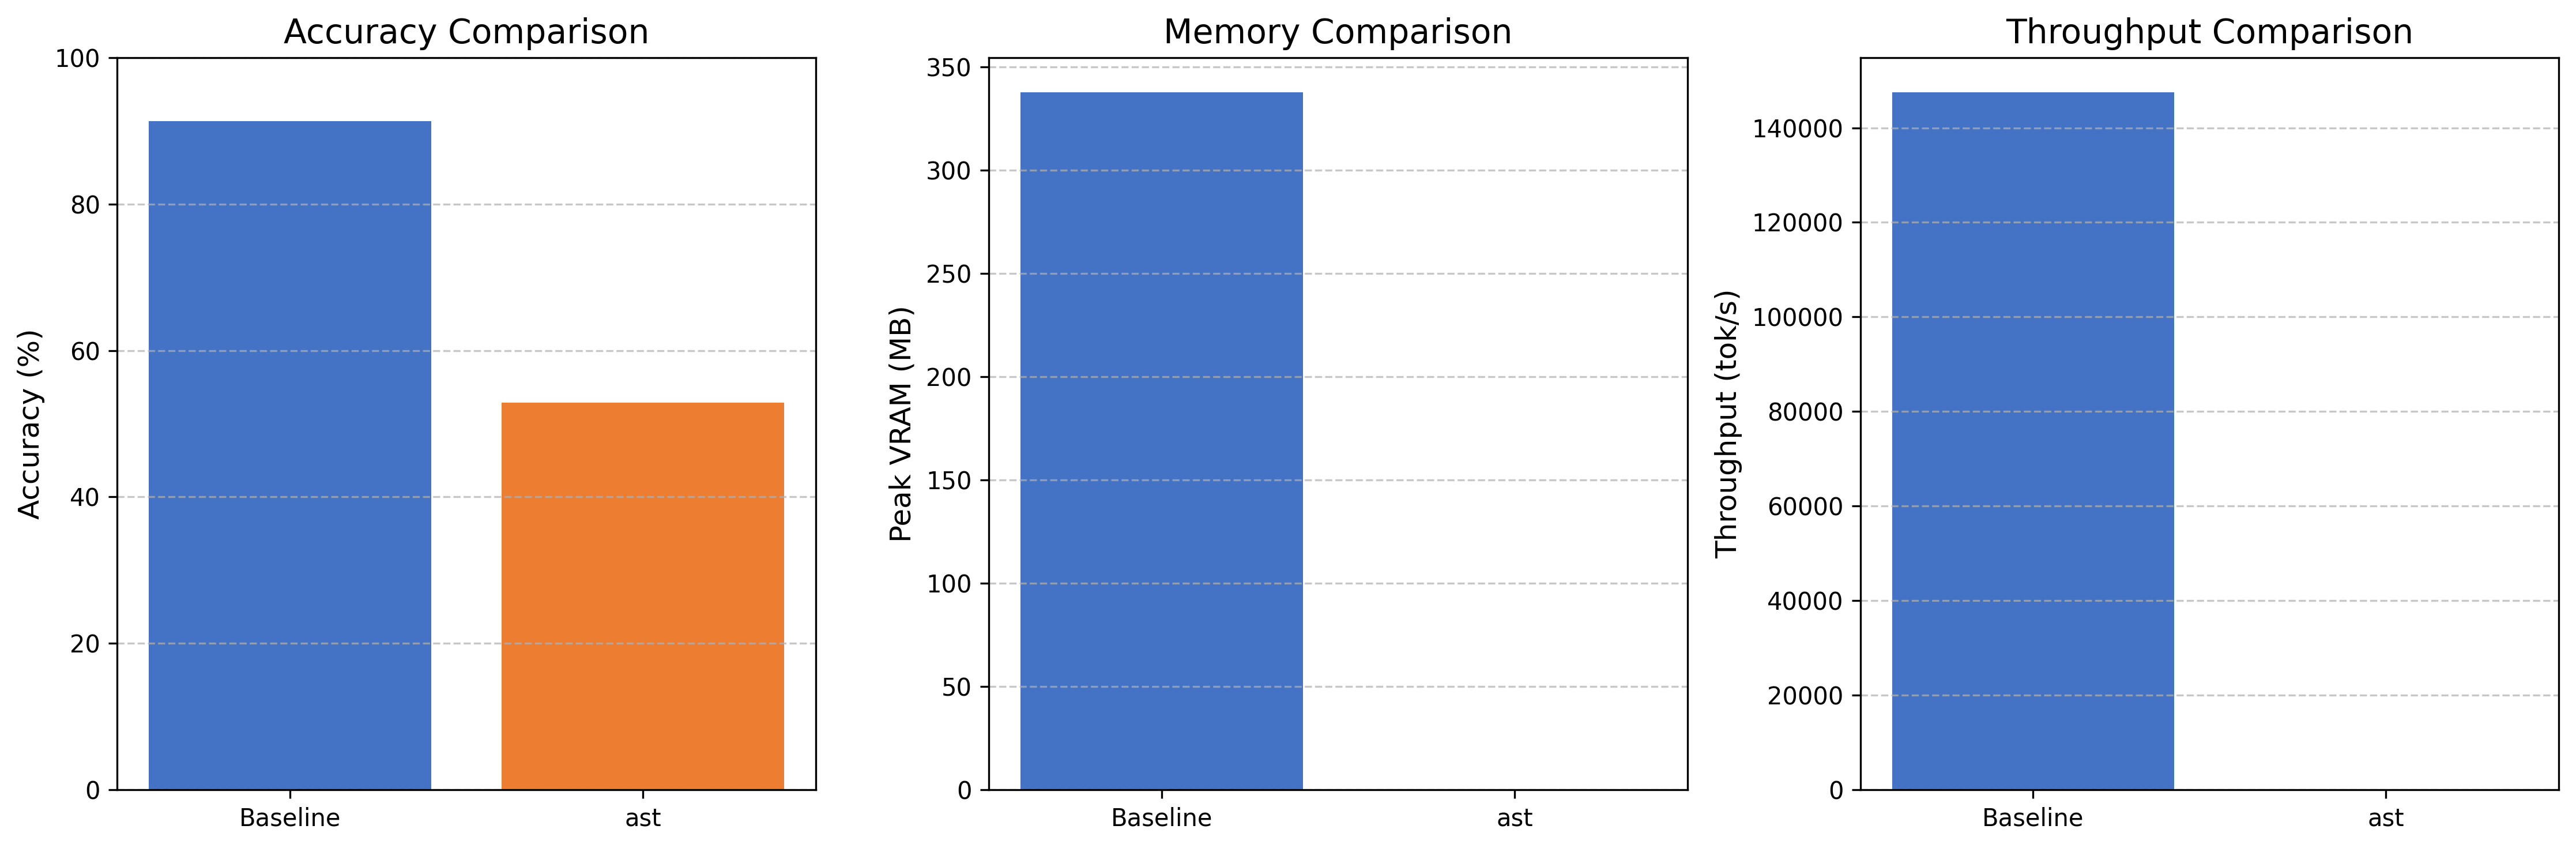
\includegraphics[width=0.92\textwidth]{img/comparison/ast_comparison.png}
\caption{نمودار ارزیابی مقایسه‌ای سه‌شاخصی دقت، اوج مصرف حافظه و توان عملیاتی مکانیزم \lr{fast\_attention} در برابر خط مبنا}
\label{fig:comp_fast_attention}
\end{figure}
